% Created by tikzDevice version 0.12.6 on 2025-02-15 05:42:56
% !TEX encoding = UTF-8 Unicode
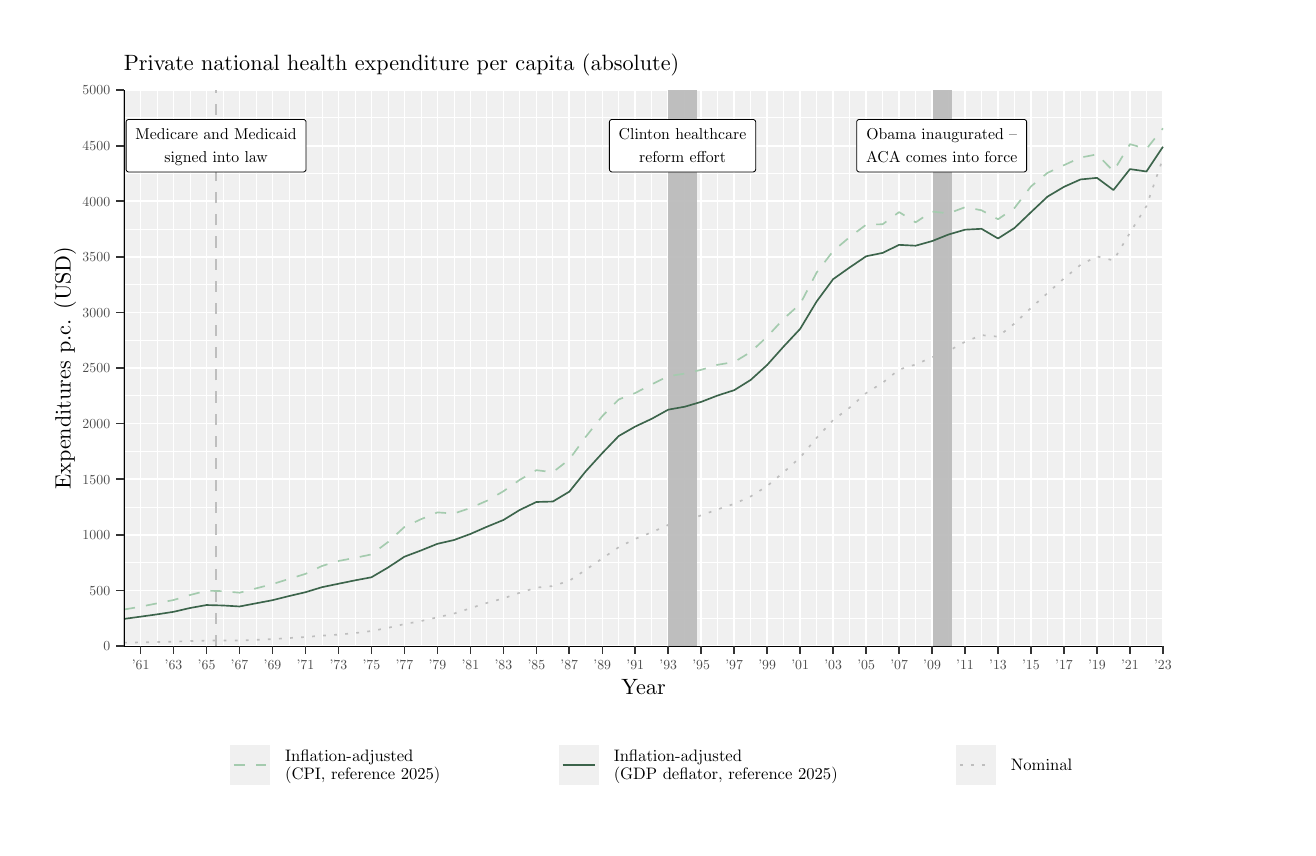
\begin{tikzpicture}[x=1pt,y=1pt]
\definecolor{fillColor}{RGB}{255,255,255}
\path[use as bounding box,fill=fillColor,fill opacity=0.00] (0,0) rectangle (455.30,289.08);
\begin{scope}
\path[clip] (  0.00,  0.00) rectangle (455.30,289.08);
\definecolor{drawColor}{RGB}{255,255,255}
\definecolor{fillColor}{RGB}{255,255,255}

\path[draw=drawColor,line width= 0.6pt,line join=round,line cap=round,fill=fillColor] (  0.00,  0.00) rectangle (455.30,289.08);
\end{scope}
\begin{scope}
\path[clip] (  0.00,  0.00) rectangle (455.30,289.08);
\definecolor{fillColor}{gray}{0.94}

\path[fill=fillColor] ( 34.76, 65.63) rectangle (410.30,266.52);
\definecolor{drawColor}{RGB}{255,255,255}

\path[draw=drawColor,line width= 0.3pt,line join=round] ( 34.76, 75.68) --
	(410.30, 75.68);

\path[draw=drawColor,line width= 0.3pt,line join=round] ( 34.76, 95.77) --
	(410.30, 95.77);

\path[draw=drawColor,line width= 0.3pt,line join=round] ( 34.76,115.85) --
	(410.30,115.85);

\path[draw=drawColor,line width= 0.3pt,line join=round] ( 34.76,135.94) --
	(410.30,135.94);

\path[draw=drawColor,line width= 0.3pt,line join=round] ( 34.76,156.03) --
	(410.30,156.03);

\path[draw=drawColor,line width= 0.3pt,line join=round] ( 34.76,176.12) --
	(410.30,176.12);

\path[draw=drawColor,line width= 0.3pt,line join=round] ( 34.76,196.21) --
	(410.30,196.21);

\path[draw=drawColor,line width= 0.3pt,line join=round] ( 34.76,216.29) --
	(410.30,216.29);

\path[draw=drawColor,line width= 0.3pt,line join=round] ( 34.76,236.38) --
	(410.30,236.38);

\path[draw=drawColor,line width= 0.3pt,line join=round] ( 34.76,256.47) --
	(410.30,256.47);

\path[draw=drawColor,line width= 0.3pt,line join=round] ( 34.85, 65.63) --
	( 34.85,266.52);

\path[draw=drawColor,line width= 0.3pt,line join=round] ( 46.77, 65.63) --
	( 46.77,266.52);

\path[draw=drawColor,line width= 0.3pt,line join=round] ( 58.69, 65.63) --
	( 58.69,266.52);

\path[draw=drawColor,line width= 0.3pt,line join=round] ( 70.60, 65.63) --
	( 70.60,266.52);

\path[draw=drawColor,line width= 0.3pt,line join=round] ( 82.52, 65.63) --
	( 82.52,266.52);

\path[draw=drawColor,line width= 0.3pt,line join=round] ( 94.43, 65.63) --
	( 94.43,266.52);

\path[draw=drawColor,line width= 0.3pt,line join=round] (106.35, 65.63) --
	(106.35,266.52);

\path[draw=drawColor,line width= 0.3pt,line join=round] (118.27, 65.63) --
	(118.27,266.52);

\path[draw=drawColor,line width= 0.3pt,line join=round] (130.18, 65.63) --
	(130.18,266.52);

\path[draw=drawColor,line width= 0.3pt,line join=round] (142.10, 65.63) --
	(142.10,266.52);

\path[draw=drawColor,line width= 0.3pt,line join=round] (154.02, 65.63) --
	(154.02,266.52);

\path[draw=drawColor,line width= 0.3pt,line join=round] (165.93, 65.63) --
	(165.93,266.52);

\path[draw=drawColor,line width= 0.3pt,line join=round] (177.85, 65.63) --
	(177.85,266.52);

\path[draw=drawColor,line width= 0.3pt,line join=round] (189.77, 65.63) --
	(189.77,266.52);

\path[draw=drawColor,line width= 0.3pt,line join=round] (201.68, 65.63) --
	(201.68,266.52);

\path[draw=drawColor,line width= 0.3pt,line join=round] (213.60, 65.63) --
	(213.60,266.52);

\path[draw=drawColor,line width= 0.3pt,line join=round] (225.52, 65.63) --
	(225.52,266.52);

\path[draw=drawColor,line width= 0.3pt,line join=round] (237.43, 65.63) --
	(237.43,266.52);

\path[draw=drawColor,line width= 0.3pt,line join=round] (249.35, 65.63) --
	(249.35,266.52);

\path[draw=drawColor,line width= 0.3pt,line join=round] (261.27, 65.63) --
	(261.27,266.52);

\path[draw=drawColor,line width= 0.3pt,line join=round] (273.18, 65.63) --
	(273.18,266.52);

\path[draw=drawColor,line width= 0.3pt,line join=round] (285.10, 65.63) --
	(285.10,266.52);

\path[draw=drawColor,line width= 0.3pt,line join=round] (297.02, 65.63) --
	(297.02,266.52);

\path[draw=drawColor,line width= 0.3pt,line join=round] (308.93, 65.63) --
	(308.93,266.52);

\path[draw=drawColor,line width= 0.3pt,line join=round] (320.85, 65.63) --
	(320.85,266.52);

\path[draw=drawColor,line width= 0.3pt,line join=round] (332.77, 65.63) --
	(332.77,266.52);

\path[draw=drawColor,line width= 0.3pt,line join=round] (344.68, 65.63) --
	(344.68,266.52);

\path[draw=drawColor,line width= 0.3pt,line join=round] (356.60, 65.63) --
	(356.60,266.52);

\path[draw=drawColor,line width= 0.3pt,line join=round] (368.52, 65.63) --
	(368.52,266.52);

\path[draw=drawColor,line width= 0.3pt,line join=round] (380.43, 65.63) --
	(380.43,266.52);

\path[draw=drawColor,line width= 0.3pt,line join=round] (392.35, 65.63) --
	(392.35,266.52);

\path[draw=drawColor,line width= 0.3pt,line join=round] (404.27, 65.63) --
	(404.27,266.52);

\path[draw=drawColor,line width= 0.6pt,line join=round] ( 34.76, 65.63) --
	(410.30, 65.63);

\path[draw=drawColor,line width= 0.6pt,line join=round] ( 34.76, 85.72) --
	(410.30, 85.72);

\path[draw=drawColor,line width= 0.6pt,line join=round] ( 34.76,105.81) --
	(410.30,105.81);

\path[draw=drawColor,line width= 0.6pt,line join=round] ( 34.76,125.90) --
	(410.30,125.90);

\path[draw=drawColor,line width= 0.6pt,line join=round] ( 34.76,145.99) --
	(410.30,145.99);

\path[draw=drawColor,line width= 0.6pt,line join=round] ( 34.76,166.07) --
	(410.30,166.07);

\path[draw=drawColor,line width= 0.6pt,line join=round] ( 34.76,186.16) --
	(410.30,186.16);

\path[draw=drawColor,line width= 0.6pt,line join=round] ( 34.76,206.25) --
	(410.30,206.25);

\path[draw=drawColor,line width= 0.6pt,line join=round] ( 34.76,226.34) --
	(410.30,226.34);

\path[draw=drawColor,line width= 0.6pt,line join=round] ( 34.76,246.43) --
	(410.30,246.43);

\path[draw=drawColor,line width= 0.6pt,line join=round] ( 34.76,266.52) --
	(410.30,266.52);

\path[draw=drawColor,line width= 0.6pt,line join=round] ( 40.81, 65.63) --
	( 40.81,266.52);

\path[draw=drawColor,line width= 0.6pt,line join=round] ( 52.72, 65.63) --
	( 52.72,266.52);

\path[draw=drawColor,line width= 0.6pt,line join=round] ( 64.65, 65.63) --
	( 64.65,266.52);

\path[draw=drawColor,line width= 0.6pt,line join=round] ( 76.56, 65.63) --
	( 76.56,266.52);

\path[draw=drawColor,line width= 0.6pt,line join=round] ( 88.48, 65.63) --
	( 88.48,266.52);

\path[draw=drawColor,line width= 0.6pt,line join=round] (100.39, 65.63) --
	(100.39,266.52);

\path[draw=drawColor,line width= 0.6pt,line join=round] (112.31, 65.63) --
	(112.31,266.52);

\path[draw=drawColor,line width= 0.6pt,line join=round] (124.22, 65.63) --
	(124.22,266.52);

\path[draw=drawColor,line width= 0.6pt,line join=round] (136.15, 65.63) --
	(136.15,266.52);

\path[draw=drawColor,line width= 0.6pt,line join=round] (148.06, 65.63) --
	(148.06,266.52);

\path[draw=drawColor,line width= 0.6pt,line join=round] (159.98, 65.63) --
	(159.98,266.52);

\path[draw=drawColor,line width= 0.6pt,line join=round] (171.89, 65.63) --
	(171.89,266.52);

\path[draw=drawColor,line width= 0.6pt,line join=round] (183.81, 65.63) --
	(183.81,266.52);

\path[draw=drawColor,line width= 0.6pt,line join=round] (195.72, 65.63) --
	(195.72,266.52);

\path[draw=drawColor,line width= 0.6pt,line join=round] (207.65, 65.63) --
	(207.65,266.52);

\path[draw=drawColor,line width= 0.6pt,line join=round] (219.55, 65.63) --
	(219.55,266.52);

\path[draw=drawColor,line width= 0.6pt,line join=round] (231.48, 65.63) --
	(231.48,266.52);

\path[draw=drawColor,line width= 0.6pt,line join=round] (243.39, 65.63) --
	(243.39,266.52);

\path[draw=drawColor,line width= 0.6pt,line join=round] (255.31, 65.63) --
	(255.31,266.52);

\path[draw=drawColor,line width= 0.6pt,line join=round] (267.22, 65.63) --
	(267.22,266.52);

\path[draw=drawColor,line width= 0.6pt,line join=round] (279.15, 65.63) --
	(279.15,266.52);

\path[draw=drawColor,line width= 0.6pt,line join=round] (291.05, 65.63) --
	(291.05,266.52);

\path[draw=drawColor,line width= 0.6pt,line join=round] (302.98, 65.63) --
	(302.98,266.52);

\path[draw=drawColor,line width= 0.6pt,line join=round] (314.89, 65.63) --
	(314.89,266.52);

\path[draw=drawColor,line width= 0.6pt,line join=round] (326.81, 65.63) --
	(326.81,266.52);

\path[draw=drawColor,line width= 0.6pt,line join=round] (338.72, 65.63) --
	(338.72,266.52);

\path[draw=drawColor,line width= 0.6pt,line join=round] (350.64, 65.63) --
	(350.64,266.52);

\path[draw=drawColor,line width= 0.6pt,line join=round] (362.55, 65.63) --
	(362.55,266.52);

\path[draw=drawColor,line width= 0.6pt,line join=round] (374.48, 65.63) --
	(374.48,266.52);

\path[draw=drawColor,line width= 0.6pt,line join=round] (386.39, 65.63) --
	(386.39,266.52);

\path[draw=drawColor,line width= 0.6pt,line join=round] (398.31, 65.63) --
	(398.31,266.52);

\path[draw=drawColor,line width= 0.6pt,line join=round] (410.22, 65.63) --
	(410.22,266.52);
\definecolor{drawColor}{RGB}{190,190,190}

\path[draw=drawColor,line width= 0.6pt,line join=round] ( 34.84, 65.63) -- ( 34.84,266.52);
\definecolor{fillColor}{RGB}{190,190,190}

\path[fill=fillColor,fill opacity=0.01] (231.48, 65.63) rectangle (241.81,266.52);

\path[fill=fillColor,fill opacity=0.01] (231.48, 65.63) rectangle (241.81,266.52);

\path[fill=fillColor,fill opacity=0.01] (231.48, 65.63) rectangle (241.81,266.52);

\path[fill=fillColor,fill opacity=0.01] (231.48, 65.63) rectangle (241.81,266.52);

\path[fill=fillColor,fill opacity=0.01] (231.48, 65.63) rectangle (241.81,266.52);

\path[fill=fillColor,fill opacity=0.01] (231.48, 65.63) rectangle (241.81,266.52);

\path[fill=fillColor,fill opacity=0.01] (231.48, 65.63) rectangle (241.81,266.52);

\path[fill=fillColor,fill opacity=0.01] (231.48, 65.63) rectangle (241.81,266.52);

\path[fill=fillColor,fill opacity=0.01] (231.48, 65.63) rectangle (241.81,266.52);

\path[fill=fillColor,fill opacity=0.01] (231.48, 65.63) rectangle (241.81,266.52);

\path[fill=fillColor,fill opacity=0.01] (231.48, 65.63) rectangle (241.81,266.52);

\path[fill=fillColor,fill opacity=0.01] (231.48, 65.63) rectangle (241.81,266.52);

\path[fill=fillColor,fill opacity=0.01] (231.48, 65.63) rectangle (241.81,266.52);

\path[fill=fillColor,fill opacity=0.01] (231.48, 65.63) rectangle (241.81,266.52);

\path[fill=fillColor,fill opacity=0.01] (231.48, 65.63) rectangle (241.81,266.52);

\path[fill=fillColor,fill opacity=0.01] (231.48, 65.63) rectangle (241.81,266.52);

\path[fill=fillColor,fill opacity=0.01] (231.48, 65.63) rectangle (241.81,266.52);

\path[fill=fillColor,fill opacity=0.01] (231.48, 65.63) rectangle (241.81,266.52);

\path[fill=fillColor,fill opacity=0.01] (231.48, 65.63) rectangle (241.81,266.52);

\path[fill=fillColor,fill opacity=0.01] (231.48, 65.63) rectangle (241.81,266.52);

\path[fill=fillColor,fill opacity=0.01] (231.48, 65.63) rectangle (241.81,266.52);

\path[fill=fillColor,fill opacity=0.01] (231.48, 65.63) rectangle (241.81,266.52);

\path[fill=fillColor,fill opacity=0.01] (231.48, 65.63) rectangle (241.81,266.52);

\path[fill=fillColor,fill opacity=0.01] (231.48, 65.63) rectangle (241.81,266.52);

\path[fill=fillColor,fill opacity=0.01] (231.48, 65.63) rectangle (241.81,266.52);

\path[fill=fillColor,fill opacity=0.01] (231.48, 65.63) rectangle (241.81,266.52);

\path[fill=fillColor,fill opacity=0.01] (231.48, 65.63) rectangle (241.81,266.52);

\path[fill=fillColor,fill opacity=0.01] (231.48, 65.63) rectangle (241.81,266.52);

\path[fill=fillColor,fill opacity=0.01] (231.48, 65.63) rectangle (241.81,266.52);

\path[fill=fillColor,fill opacity=0.01] (231.48, 65.63) rectangle (241.81,266.52);

\path[fill=fillColor,fill opacity=0.01] (231.48, 65.63) rectangle (241.81,266.52);

\path[fill=fillColor,fill opacity=0.01] (231.48, 65.63) rectangle (241.81,266.52);

\path[fill=fillColor,fill opacity=0.01] (231.48, 65.63) rectangle (241.81,266.52);

\path[fill=fillColor,fill opacity=0.01] (231.48, 65.63) rectangle (241.81,266.52);

\path[fill=fillColor,fill opacity=0.01] (231.48, 65.63) rectangle (241.81,266.52);

\path[fill=fillColor,fill opacity=0.01] (231.48, 65.63) rectangle (241.81,266.52);

\path[fill=fillColor,fill opacity=0.01] (231.48, 65.63) rectangle (241.81,266.52);

\path[fill=fillColor,fill opacity=0.01] (231.48, 65.63) rectangle (241.81,266.52);

\path[fill=fillColor,fill opacity=0.01] (231.48, 65.63) rectangle (241.81,266.52);

\path[fill=fillColor,fill opacity=0.01] (231.48, 65.63) rectangle (241.81,266.52);

\path[fill=fillColor,fill opacity=0.01] (231.48, 65.63) rectangle (241.81,266.52);

\path[fill=fillColor,fill opacity=0.01] (231.48, 65.63) rectangle (241.81,266.52);

\path[fill=fillColor,fill opacity=0.01] (231.48, 65.63) rectangle (241.81,266.52);

\path[fill=fillColor,fill opacity=0.01] (231.48, 65.63) rectangle (241.81,266.52);

\path[fill=fillColor,fill opacity=0.01] (231.48, 65.63) rectangle (241.81,266.52);

\path[fill=fillColor,fill opacity=0.01] (231.48, 65.63) rectangle (241.81,266.52);

\path[fill=fillColor,fill opacity=0.01] (231.48, 65.63) rectangle (241.81,266.52);

\path[fill=fillColor,fill opacity=0.01] (231.48, 65.63) rectangle (241.81,266.52);

\path[fill=fillColor,fill opacity=0.01] (231.48, 65.63) rectangle (241.81,266.52);

\path[fill=fillColor,fill opacity=0.01] (231.48, 65.63) rectangle (241.81,266.52);

\path[fill=fillColor,fill opacity=0.01] (231.48, 65.63) rectangle (241.81,266.52);

\path[fill=fillColor,fill opacity=0.01] (231.48, 65.63) rectangle (241.81,266.52);

\path[fill=fillColor,fill opacity=0.01] (231.48, 65.63) rectangle (241.81,266.52);

\path[fill=fillColor,fill opacity=0.01] (231.48, 65.63) rectangle (241.81,266.52);

\path[fill=fillColor,fill opacity=0.01] (231.48, 65.63) rectangle (241.81,266.52);

\path[fill=fillColor,fill opacity=0.01] (231.48, 65.63) rectangle (241.81,266.52);

\path[fill=fillColor,fill opacity=0.01] (231.48, 65.63) rectangle (241.81,266.52);

\path[fill=fillColor,fill opacity=0.01] (231.48, 65.63) rectangle (241.81,266.52);

\path[fill=fillColor,fill opacity=0.01] (231.48, 65.63) rectangle (241.81,266.52);

\path[fill=fillColor,fill opacity=0.01] (231.48, 65.63) rectangle (241.81,266.52);

\path[fill=fillColor,fill opacity=0.01] (231.48, 65.63) rectangle (241.81,266.52);

\path[fill=fillColor,fill opacity=0.01] (231.48, 65.63) rectangle (241.81,266.52);

\path[fill=fillColor,fill opacity=0.01] (231.48, 65.63) rectangle (241.81,266.52);

\path[fill=fillColor,fill opacity=0.01] (231.48, 65.63) rectangle (241.81,266.52);

\path[fill=fillColor,fill opacity=0.01] (327.12, 65.63) rectangle (334.09,266.52);

\path[fill=fillColor,fill opacity=0.01] (327.12, 65.63) rectangle (334.09,266.52);

\path[fill=fillColor,fill opacity=0.01] (327.12, 65.63) rectangle (334.09,266.52);

\path[fill=fillColor,fill opacity=0.01] (327.12, 65.63) rectangle (334.09,266.52);

\path[fill=fillColor,fill opacity=0.01] (327.12, 65.63) rectangle (334.09,266.52);

\path[fill=fillColor,fill opacity=0.01] (327.12, 65.63) rectangle (334.09,266.52);

\path[fill=fillColor,fill opacity=0.01] (327.12, 65.63) rectangle (334.09,266.52);

\path[fill=fillColor,fill opacity=0.01] (327.12, 65.63) rectangle (334.09,266.52);

\path[fill=fillColor,fill opacity=0.01] (327.12, 65.63) rectangle (334.09,266.52);

\path[fill=fillColor,fill opacity=0.01] (327.12, 65.63) rectangle (334.09,266.52);

\path[fill=fillColor,fill opacity=0.01] (327.12, 65.63) rectangle (334.09,266.52);

\path[fill=fillColor,fill opacity=0.01] (327.12, 65.63) rectangle (334.09,266.52);

\path[fill=fillColor,fill opacity=0.01] (327.12, 65.63) rectangle (334.09,266.52);

\path[fill=fillColor,fill opacity=0.01] (327.12, 65.63) rectangle (334.09,266.52);

\path[fill=fillColor,fill opacity=0.01] (327.12, 65.63) rectangle (334.09,266.52);

\path[fill=fillColor,fill opacity=0.01] (327.12, 65.63) rectangle (334.09,266.52);

\path[fill=fillColor,fill opacity=0.01] (327.12, 65.63) rectangle (334.09,266.52);

\path[fill=fillColor,fill opacity=0.01] (327.12, 65.63) rectangle (334.09,266.52);

\path[fill=fillColor,fill opacity=0.01] (327.12, 65.63) rectangle (334.09,266.52);

\path[fill=fillColor,fill opacity=0.01] (327.12, 65.63) rectangle (334.09,266.52);

\path[fill=fillColor,fill opacity=0.01] (327.12, 65.63) rectangle (334.09,266.52);

\path[fill=fillColor,fill opacity=0.01] (327.12, 65.63) rectangle (334.09,266.52);

\path[fill=fillColor,fill opacity=0.01] (327.12, 65.63) rectangle (334.09,266.52);

\path[fill=fillColor,fill opacity=0.01] (327.12, 65.63) rectangle (334.09,266.52);

\path[fill=fillColor,fill opacity=0.01] (327.12, 65.63) rectangle (334.09,266.52);

\path[fill=fillColor,fill opacity=0.01] (327.12, 65.63) rectangle (334.09,266.52);

\path[fill=fillColor,fill opacity=0.01] (327.12, 65.63) rectangle (334.09,266.52);

\path[fill=fillColor,fill opacity=0.01] (327.12, 65.63) rectangle (334.09,266.52);

\path[fill=fillColor,fill opacity=0.01] (327.12, 65.63) rectangle (334.09,266.52);

\path[fill=fillColor,fill opacity=0.01] (327.12, 65.63) rectangle (334.09,266.52);

\path[fill=fillColor,fill opacity=0.01] (327.12, 65.63) rectangle (334.09,266.52);

\path[fill=fillColor,fill opacity=0.01] (327.12, 65.63) rectangle (334.09,266.52);

\path[fill=fillColor,fill opacity=0.01] (327.12, 65.63) rectangle (334.09,266.52);

\path[fill=fillColor,fill opacity=0.01] (327.12, 65.63) rectangle (334.09,266.52);

\path[fill=fillColor,fill opacity=0.01] (327.12, 65.63) rectangle (334.09,266.52);

\path[fill=fillColor,fill opacity=0.01] (327.12, 65.63) rectangle (334.09,266.52);

\path[fill=fillColor,fill opacity=0.01] (327.12, 65.63) rectangle (334.09,266.52);

\path[fill=fillColor,fill opacity=0.01] (327.12, 65.63) rectangle (334.09,266.52);

\path[fill=fillColor,fill opacity=0.01] (327.12, 65.63) rectangle (334.09,266.52);

\path[fill=fillColor,fill opacity=0.01] (327.12, 65.63) rectangle (334.09,266.52);

\path[fill=fillColor,fill opacity=0.01] (327.12, 65.63) rectangle (334.09,266.52);

\path[fill=fillColor,fill opacity=0.01] (327.12, 65.63) rectangle (334.09,266.52);

\path[fill=fillColor,fill opacity=0.01] (327.12, 65.63) rectangle (334.09,266.52);

\path[fill=fillColor,fill opacity=0.01] (327.12, 65.63) rectangle (334.09,266.52);

\path[fill=fillColor,fill opacity=0.01] (327.12, 65.63) rectangle (334.09,266.52);

\path[fill=fillColor,fill opacity=0.01] (327.12, 65.63) rectangle (334.09,266.52);

\path[fill=fillColor,fill opacity=0.01] (327.12, 65.63) rectangle (334.09,266.52);

\path[fill=fillColor,fill opacity=0.01] (327.12, 65.63) rectangle (334.09,266.52);

\path[fill=fillColor,fill opacity=0.01] (327.12, 65.63) rectangle (334.09,266.52);

\path[fill=fillColor,fill opacity=0.01] (327.12, 65.63) rectangle (334.09,266.52);

\path[fill=fillColor,fill opacity=0.01] (327.12, 65.63) rectangle (334.09,266.52);

\path[fill=fillColor,fill opacity=0.01] (327.12, 65.63) rectangle (334.09,266.52);

\path[fill=fillColor,fill opacity=0.01] (327.12, 65.63) rectangle (334.09,266.52);

\path[fill=fillColor,fill opacity=0.01] (327.12, 65.63) rectangle (334.09,266.52);

\path[fill=fillColor,fill opacity=0.01] (327.12, 65.63) rectangle (334.09,266.52);

\path[fill=fillColor,fill opacity=0.01] (327.12, 65.63) rectangle (334.09,266.52);

\path[fill=fillColor,fill opacity=0.01] (327.12, 65.63) rectangle (334.09,266.52);

\path[fill=fillColor,fill opacity=0.01] (327.12, 65.63) rectangle (334.09,266.52);

\path[fill=fillColor,fill opacity=0.01] (327.12, 65.63) rectangle (334.09,266.52);

\path[fill=fillColor,fill opacity=0.01] (327.12, 65.63) rectangle (334.09,266.52);

\path[fill=fillColor,fill opacity=0.01] (327.12, 65.63) rectangle (334.09,266.52);

\path[fill=fillColor,fill opacity=0.01] (327.12, 65.63) rectangle (334.09,266.52);

\path[fill=fillColor,fill opacity=0.01] (327.12, 65.63) rectangle (334.09,266.52);

\path[fill=fillColor,fill opacity=0.01] (327.12, 65.63) rectangle (334.09,266.52);

\path[draw=drawColor,line width= 0.6pt,dash pattern=on 4pt off 4pt ,line join=round] ( 68.07, 65.63) -- ( 68.07,266.52);
\definecolor{drawColor}{RGB}{0,0,0}
\definecolor{fillColor}{RGB}{255,255,255}

\path[draw=drawColor,line width= 0.3pt,line join=round,line cap=round,fill=fillColor] ( 36.59,236.94) --
	( 99.56,236.94) --
	( 99.52,236.94) --
	( 99.68,236.95) --
	( 99.85,236.98) --
	(100.00,237.04) --
	(100.14,237.12) --
	(100.27,237.23) --
	(100.38,237.35) --
	(100.47,237.49) --
	(100.54,237.65) --
	(100.58,237.81) --
	(100.59,237.97) --
	(100.59,237.97) --
	(100.59,254.88) --
	(100.59,254.88) --
	(100.58,255.05) --
	(100.54,255.21) --
	(100.47,255.36) --
	(100.38,255.50) --
	(100.27,255.62) --
	(100.14,255.73) --
	(100.00,255.81) --
	( 99.85,255.87) --
	( 99.68,255.90) --
	( 99.56,255.91) --
	( 36.59,255.91) --
	( 36.71,255.90) --
	( 36.54,255.91) --
	( 36.38,255.89) --
	( 36.22,255.84) --
	( 36.07,255.77) --
	( 35.94,255.68) --
	( 35.82,255.56) --
	( 35.72,255.43) --
	( 35.64,255.29) --
	( 35.59,255.13) --
	( 35.56,254.97) --
	( 35.56,254.88) --
	( 35.56,237.97) --
	( 35.56,238.05) --
	( 35.56,237.89) --
	( 35.59,237.72) --
	( 35.64,237.57) --
	( 35.72,237.42) --
	( 35.82,237.29) --
	( 35.94,237.17) --
	( 36.07,237.08) --
	( 36.22,237.01) --
	( 36.38,236.96) --
	( 36.54,236.94) --
	cycle;
\end{scope}
\begin{scope}
\path[clip] (  0.00,  0.00) rectangle (455.30,289.08);
\definecolor{drawColor}{RGB}{0,0,0}

\node[text=drawColor,anchor=base,inner sep=0pt, outer sep=0pt, scale=  0.57] at ( 68.07,248.56) {Medicare and Medicaid };

\node[text=drawColor,anchor=base,inner sep=0pt, outer sep=0pt, scale=  0.57] at ( 68.07,240.37) { signed into law};
\end{scope}
\begin{scope}
\path[clip] (  0.00,  0.00) rectangle (455.30,289.08);
\definecolor{drawColor}{RGB}{0,0,0}
\definecolor{fillColor}{RGB}{255,255,255}

\path[draw=drawColor,line width= 0.3pt,line join=round,line cap=round,fill=fillColor] (211.23,236.94) --
	(262.04,236.94) --
	(262.00,236.94) --
	(262.16,236.95) --
	(262.32,236.98) --
	(262.48,237.04) --
	(262.62,237.12) --
	(262.75,237.23) --
	(262.86,237.35) --
	(262.95,237.49) --
	(263.01,237.65) --
	(263.05,237.81) --
	(263.07,237.97) --
	(263.07,237.97) --
	(263.07,254.88) --
	(263.07,254.88) --
	(263.05,255.05) --
	(263.01,255.21) --
	(262.95,255.36) --
	(262.86,255.50) --
	(262.75,255.62) --
	(262.62,255.73) --
	(262.48,255.81) --
	(262.32,255.87) --
	(262.16,255.90) --
	(262.04,255.91) --
	(211.23,255.91) --
	(211.36,255.90) --
	(211.19,255.91) --
	(211.03,255.89) --
	(210.87,255.84) --
	(210.72,255.77) --
	(210.58,255.68) --
	(210.46,255.56) --
	(210.36,255.43) --
	(210.29,255.29) --
	(210.23,255.13) --
	(210.21,254.97) --
	(210.20,254.88) --
	(210.20,237.97) --
	(210.21,238.05) --
	(210.21,237.89) --
	(210.23,237.72) --
	(210.29,237.57) --
	(210.36,237.42) --
	(210.46,237.29) --
	(210.58,237.17) --
	(210.72,237.08) --
	(210.87,237.01) --
	(211.03,236.96) --
	(211.19,236.94) --
	cycle;
\end{scope}
\begin{scope}
\path[clip] (  0.00,  0.00) rectangle (455.30,289.08);
\definecolor{drawColor}{RGB}{0,0,0}

\node[text=drawColor,anchor=base,inner sep=0pt, outer sep=0pt, scale=  0.57] at (236.63,248.56) {Clinton healthcare };

\node[text=drawColor,anchor=base,inner sep=0pt, outer sep=0pt, scale=  0.57] at (236.63,240.37) { reform effort};
\end{scope}
\begin{scope}
\path[clip] (  0.00,  0.00) rectangle (455.30,289.08);
\definecolor{drawColor}{RGB}{0,0,0}
\definecolor{fillColor}{RGB}{255,255,255}

\path[draw=drawColor,line width= 0.3pt,line join=round,line cap=round,fill=fillColor] (300.58,236.94) --
	(359.96,236.94) --
	(359.91,236.94) --
	(360.08,236.95) --
	(360.24,236.98) --
	(360.40,237.04) --
	(360.54,237.12) --
	(360.67,237.23) --
	(360.78,237.35) --
	(360.87,237.49) --
	(360.93,237.65) --
	(360.97,237.81) --
	(360.98,237.97) --
	(360.98,237.97) --
	(360.98,254.88) --
	(360.98,254.88) --
	(360.97,255.05) --
	(360.93,255.21) --
	(360.87,255.36) --
	(360.78,255.50) --
	(360.67,255.62) --
	(360.54,255.73) --
	(360.40,255.81) --
	(360.24,255.87) --
	(360.08,255.90) --
	(359.96,255.91) --
	(300.58,255.91) --
	(300.71,255.90) --
	(300.54,255.91) --
	(300.38,255.89) --
	(300.22,255.84) --
	(300.07,255.77) --
	(299.93,255.68) --
	(299.81,255.56) --
	(299.72,255.43) --
	(299.64,255.29) --
	(299.59,255.13) --
	(299.56,254.97) --
	(299.56,254.88) --
	(299.56,237.97) --
	(299.56,238.05) --
	(299.56,237.89) --
	(299.59,237.72) --
	(299.64,237.57) --
	(299.72,237.42) --
	(299.81,237.29) --
	(299.93,237.17) --
	(300.07,237.08) --
	(300.22,237.01) --
	(300.38,236.96) --
	(300.54,236.94) --
	cycle;
\end{scope}
\begin{scope}
\path[clip] (  0.00,  0.00) rectangle (455.30,289.08);
\definecolor{drawColor}{RGB}{0,0,0}

\node[text=drawColor,anchor=base,inner sep=0pt, outer sep=0pt, scale=  0.57] at (330.27,248.56) {Obama inaugurated -- };

\node[text=drawColor,anchor=base,inner sep=0pt, outer sep=0pt, scale=  0.57] at (330.27,240.37) { ACA comes into force};
\end{scope}
\begin{scope}
\path[clip] (  0.00,  0.00) rectangle (455.30,289.08);
\definecolor{drawColor}{RGB}{190,190,190}

\path[draw=drawColor,line width= 0.6pt,dash pattern=on 1pt off 3pt ,line join=round] ( 34.84, 66.85) --
	( 40.81, 66.97) --
	( 46.77, 67.09) --
	( 52.72, 67.23) --
	( 58.68, 67.43) --
	( 64.65, 67.60) --
	( 70.60, 67.62) --
	( 76.56, 67.63) --
	( 82.51, 67.87) --
	( 88.48, 68.14) --
	( 94.43, 68.52) --
	(100.39, 68.90) --
	(106.34, 69.38) --
	(112.31, 69.76) --
	(118.27, 70.31) --
	(124.22, 71.06) --
	(130.18, 72.21) --
	(136.15, 73.56) --
	(142.10, 74.65) --
	(148.06, 76.02) --
	(154.01, 77.36) --
	(159.98, 79.30) --
	(165.93, 81.21) --
	(171.89, 82.85) --
	(177.84, 84.90) --
	(183.81, 86.74) --
	(189.77, 87.30) --
	(195.72, 89.24) --
	(201.68, 93.19) --
	(207.65, 97.31) --
	(213.60,101.37) --
	(219.55,104.37) --
	(225.51,106.74) --
	(231.48,109.40) --
	(237.43,110.94) --
	(243.39,112.86) --
	(249.34,115.03) --
	(255.31,117.03) --
	(261.27,119.69) --
	(267.22,123.46) --
	(273.18,128.46) --
	(279.15,133.78) --
	(285.10,140.88) --
	(291.05,147.27) --
	(297.01,151.78) --
	(302.98,157.03) --
	(308.93,160.77) --
	(314.89,165.55) --
	(320.84,167.36) --
	(326.81,169.98) --
	(332.77,172.27) --
	(338.72,175.57) --
	(344.67,177.98) --
	(350.64,177.43) --
	(356.60,182.19) --
	(362.55,187.82) --
	(368.51,193.15) --
	(374.48,198.47) --
	(380.43,203.35) --
	(386.39,206.42) --
	(392.34,204.97) --
	(398.31,214.97) --
	(404.27,224.62) --
	(410.22,241.81);
\definecolor{drawColor}{RGB}{164,203,174}

\path[draw=drawColor,line width= 0.6pt,dash pattern=on 4pt off 4pt ,line join=round] ( 34.84, 78.84) --
	( 40.81, 79.85) --
	( 46.77, 81.06) --
	( 52.72, 82.26) --
	( 58.68, 84.07) --
	( 64.65, 85.62) --
	( 70.60, 85.46) --
	( 76.56, 84.90) --
	( 82.51, 86.46) --
	( 88.48, 88.02) --
	( 94.43, 89.88) --
	(100.39, 91.71) --
	(106.34, 94.56) --
	(112.31, 96.37) --
	(118.27, 97.49) --
	(124.22, 98.74) --
	(130.18,103.18) --
	(136.15,108.66) --
	(142.10,111.45) --
	(148.06,113.93) --
	(154.01,113.50) --
	(159.98,115.52) --
	(165.93,118.12) --
	(171.89,121.55) --
	(177.84,125.70) --
	(183.81,129.18) --
	(189.77,128.44) --
	(195.72,133.06) --
	(201.68,141.28) --
	(207.65,148.72) --
	(213.60,154.74) --
	(219.55,157.06) --
	(225.51,160.20) --
	(231.48,163.14) --
	(237.43,164.07) --
	(243.39,165.45) --
	(249.34,167.27) --
	(255.31,168.26) --
	(261.27,171.89) --
	(267.22,177.43) --
	(273.18,183.88) --
	(279.15,189.26) --
	(285.10,200.61) --
	(291.05,208.36) --
	(297.01,213.39) --
	(302.98,217.89) --
	(308.93,218.04) --
	(314.89,222.44) --
	(320.84,218.73) --
	(326.81,222.63) --
	(332.77,221.97) --
	(338.72,224.21) --
	(344.67,223.09) --
	(350.64,219.85) --
	(356.60,223.92) --
	(362.55,231.72) --
	(368.51,236.61) --
	(374.48,239.40) --
	(380.43,242.13) --
	(386.39,243.31) --
	(392.34,237.21) --
	(398.31,246.99) --
	(404.27,245.27) --
	(410.22,252.71);
\definecolor{drawColor}{RGB}{60,100,75}

\path[draw=drawColor,line width= 0.6pt,line join=round] ( 34.84, 75.44) --
	( 40.81, 76.25) --
	( 46.77, 77.08) --
	( 52.72, 78.00) --
	( 58.68, 79.38) --
	( 64.65, 80.45) --
	( 70.60, 80.29) --
	( 76.56, 79.93) --
	( 82.51, 81.07) --
	( 88.48, 82.20) --
	( 94.43, 83.69) --
	(100.39, 85.08) --
	(106.34, 86.90) --
	(112.31, 88.14) --
	(118.27, 89.36) --
	(124.22, 90.48) --
	(130.18, 93.98) --
	(136.15, 97.92) --
	(142.10,100.16) --
	(148.06,102.57) --
	(154.01,103.93) --
	(159.98,106.13) --
	(165.93,108.73) --
	(171.89,111.17) --
	(177.84,114.82) --
	(183.81,117.68) --
	(189.77,117.85) --
	(195.72,121.41) --
	(201.68,128.80) --
	(207.65,135.36) --
	(213.60,141.54) --
	(219.55,144.95) --
	(225.51,147.75) --
	(231.48,151.05) --
	(237.43,152.11) --
	(243.39,153.87) --
	(249.34,156.17) --
	(255.31,158.09) --
	(261.27,161.80) --
	(267.22,167.21) --
	(273.18,173.88) --
	(279.15,180.25) --
	(285.10,190.16) --
	(291.05,198.20) --
	(297.01,202.42) --
	(302.98,206.47) --
	(308.93,207.69) --
	(314.89,210.60) --
	(320.84,210.29) --
	(326.81,211.96) --
	(332.77,214.34) --
	(338.72,216.08) --
	(344.67,216.40) --
	(350.64,212.90) --
	(356.60,216.71) --
	(362.55,222.41) --
	(368.51,228.02) --
	(374.48,231.57) --
	(380.43,234.23) --
	(386.39,234.81) --
	(392.34,230.40) --
	(398.31,237.97) --
	(404.27,237.11) --
	(410.22,246.04);
\end{scope}
\begin{scope}
\path[clip] (  0.00,  0.00) rectangle (455.30,289.08);
\definecolor{drawColor}{RGB}{0,0,0}

\path[draw=drawColor,line width= 0.2pt,line join=round] ( 34.76, 65.63) --
	( 34.76,266.52);
\end{scope}
\begin{scope}
\path[clip] (  0.00,  0.00) rectangle (455.30,289.08);
\definecolor{drawColor}{gray}{0.30}

\node[text=drawColor,anchor=base east,inner sep=0pt, outer sep=0pt, scale=  0.50] at ( 29.81, 63.91) {0};

\node[text=drawColor,anchor=base east,inner sep=0pt, outer sep=0pt, scale=  0.50] at ( 29.81, 84.00) {500};

\node[text=drawColor,anchor=base east,inner sep=0pt, outer sep=0pt, scale=  0.50] at ( 29.81,104.09) {1000};

\node[text=drawColor,anchor=base east,inner sep=0pt, outer sep=0pt, scale=  0.50] at ( 29.81,124.18) {1500};

\node[text=drawColor,anchor=base east,inner sep=0pt, outer sep=0pt, scale=  0.50] at ( 29.81,144.26) {2000};

\node[text=drawColor,anchor=base east,inner sep=0pt, outer sep=0pt, scale=  0.50] at ( 29.81,164.35) {2500};

\node[text=drawColor,anchor=base east,inner sep=0pt, outer sep=0pt, scale=  0.50] at ( 29.81,184.44) {3000};

\node[text=drawColor,anchor=base east,inner sep=0pt, outer sep=0pt, scale=  0.50] at ( 29.81,204.53) {3500};

\node[text=drawColor,anchor=base east,inner sep=0pt, outer sep=0pt, scale=  0.50] at ( 29.81,224.62) {4000};

\node[text=drawColor,anchor=base east,inner sep=0pt, outer sep=0pt, scale=  0.50] at ( 29.81,244.71) {4500};

\node[text=drawColor,anchor=base east,inner sep=0pt, outer sep=0pt, scale=  0.50] at ( 29.81,264.79) {5000};
\end{scope}
\begin{scope}
\path[clip] (  0.00,  0.00) rectangle (455.30,289.08);
\definecolor{drawColor}{gray}{0.20}

\path[draw=drawColor,line width= 0.6pt,line join=round] ( 32.01, 65.63) --
	( 34.76, 65.63);

\path[draw=drawColor,line width= 0.6pt,line join=round] ( 32.01, 85.72) --
	( 34.76, 85.72);

\path[draw=drawColor,line width= 0.6pt,line join=round] ( 32.01,105.81) --
	( 34.76,105.81);

\path[draw=drawColor,line width= 0.6pt,line join=round] ( 32.01,125.90) --
	( 34.76,125.90);

\path[draw=drawColor,line width= 0.6pt,line join=round] ( 32.01,145.99) --
	( 34.76,145.99);

\path[draw=drawColor,line width= 0.6pt,line join=round] ( 32.01,166.07) --
	( 34.76,166.07);

\path[draw=drawColor,line width= 0.6pt,line join=round] ( 32.01,186.16) --
	( 34.76,186.16);

\path[draw=drawColor,line width= 0.6pt,line join=round] ( 32.01,206.25) --
	( 34.76,206.25);

\path[draw=drawColor,line width= 0.6pt,line join=round] ( 32.01,226.34) --
	( 34.76,226.34);

\path[draw=drawColor,line width= 0.6pt,line join=round] ( 32.01,246.43) --
	( 34.76,246.43);

\path[draw=drawColor,line width= 0.6pt,line join=round] ( 32.01,266.52) --
	( 34.76,266.52);
\end{scope}
\begin{scope}
\path[clip] (  0.00,  0.00) rectangle (455.30,289.08);
\definecolor{drawColor}{RGB}{0,0,0}

\path[draw=drawColor,line width= 0.2pt,line join=round] ( 34.76, 65.63) --
	(410.30, 65.63);
\end{scope}
\begin{scope}
\path[clip] (  0.00,  0.00) rectangle (455.30,289.08);
\definecolor{drawColor}{gray}{0.20}

\path[draw=drawColor,line width= 0.6pt,line join=round] ( 40.81, 62.88) --
	( 40.81, 65.63);

\path[draw=drawColor,line width= 0.6pt,line join=round] ( 52.72, 62.88) --
	( 52.72, 65.63);

\path[draw=drawColor,line width= 0.6pt,line join=round] ( 64.65, 62.88) --
	( 64.65, 65.63);

\path[draw=drawColor,line width= 0.6pt,line join=round] ( 76.56, 62.88) --
	( 76.56, 65.63);

\path[draw=drawColor,line width= 0.6pt,line join=round] ( 88.48, 62.88) --
	( 88.48, 65.63);

\path[draw=drawColor,line width= 0.6pt,line join=round] (100.39, 62.88) --
	(100.39, 65.63);

\path[draw=drawColor,line width= 0.6pt,line join=round] (112.31, 62.88) --
	(112.31, 65.63);

\path[draw=drawColor,line width= 0.6pt,line join=round] (124.22, 62.88) --
	(124.22, 65.63);

\path[draw=drawColor,line width= 0.6pt,line join=round] (136.15, 62.88) --
	(136.15, 65.63);

\path[draw=drawColor,line width= 0.6pt,line join=round] (148.06, 62.88) --
	(148.06, 65.63);

\path[draw=drawColor,line width= 0.6pt,line join=round] (159.98, 62.88) --
	(159.98, 65.63);

\path[draw=drawColor,line width= 0.6pt,line join=round] (171.89, 62.88) --
	(171.89, 65.63);

\path[draw=drawColor,line width= 0.6pt,line join=round] (183.81, 62.88) --
	(183.81, 65.63);

\path[draw=drawColor,line width= 0.6pt,line join=round] (195.72, 62.88) --
	(195.72, 65.63);

\path[draw=drawColor,line width= 0.6pt,line join=round] (207.65, 62.88) --
	(207.65, 65.63);

\path[draw=drawColor,line width= 0.6pt,line join=round] (219.55, 62.88) --
	(219.55, 65.63);

\path[draw=drawColor,line width= 0.6pt,line join=round] (231.48, 62.88) --
	(231.48, 65.63);

\path[draw=drawColor,line width= 0.6pt,line join=round] (243.39, 62.88) --
	(243.39, 65.63);

\path[draw=drawColor,line width= 0.6pt,line join=round] (255.31, 62.88) --
	(255.31, 65.63);

\path[draw=drawColor,line width= 0.6pt,line join=round] (267.22, 62.88) --
	(267.22, 65.63);

\path[draw=drawColor,line width= 0.6pt,line join=round] (279.15, 62.88) --
	(279.15, 65.63);

\path[draw=drawColor,line width= 0.6pt,line join=round] (291.05, 62.88) --
	(291.05, 65.63);

\path[draw=drawColor,line width= 0.6pt,line join=round] (302.98, 62.88) --
	(302.98, 65.63);

\path[draw=drawColor,line width= 0.6pt,line join=round] (314.89, 62.88) --
	(314.89, 65.63);

\path[draw=drawColor,line width= 0.6pt,line join=round] (326.81, 62.88) --
	(326.81, 65.63);

\path[draw=drawColor,line width= 0.6pt,line join=round] (338.72, 62.88) --
	(338.72, 65.63);

\path[draw=drawColor,line width= 0.6pt,line join=round] (350.64, 62.88) --
	(350.64, 65.63);

\path[draw=drawColor,line width= 0.6pt,line join=round] (362.55, 62.88) --
	(362.55, 65.63);

\path[draw=drawColor,line width= 0.6pt,line join=round] (374.48, 62.88) --
	(374.48, 65.63);

\path[draw=drawColor,line width= 0.6pt,line join=round] (386.39, 62.88) --
	(386.39, 65.63);

\path[draw=drawColor,line width= 0.6pt,line join=round] (398.31, 62.88) --
	(398.31, 65.63);

\path[draw=drawColor,line width= 0.6pt,line join=round] (410.22, 62.88) --
	(410.22, 65.63);
\end{scope}
\begin{scope}
\path[clip] (  0.00,  0.00) rectangle (455.30,289.08);
\definecolor{drawColor}{gray}{0.30}

\node[text=drawColor,anchor=base,inner sep=0pt, outer sep=0pt, scale=  0.50] at ( 40.81, 57.24) {'61};

\node[text=drawColor,anchor=base,inner sep=0pt, outer sep=0pt, scale=  0.50] at ( 52.72, 57.24) {'63};

\node[text=drawColor,anchor=base,inner sep=0pt, outer sep=0pt, scale=  0.50] at ( 64.65, 57.24) {'65};

\node[text=drawColor,anchor=base,inner sep=0pt, outer sep=0pt, scale=  0.50] at ( 76.56, 57.24) {'67};

\node[text=drawColor,anchor=base,inner sep=0pt, outer sep=0pt, scale=  0.50] at ( 88.48, 57.24) {'69};

\node[text=drawColor,anchor=base,inner sep=0pt, outer sep=0pt, scale=  0.50] at (100.39, 57.24) {'71};

\node[text=drawColor,anchor=base,inner sep=0pt, outer sep=0pt, scale=  0.50] at (112.31, 57.24) {'73};

\node[text=drawColor,anchor=base,inner sep=0pt, outer sep=0pt, scale=  0.50] at (124.22, 57.24) {'75};

\node[text=drawColor,anchor=base,inner sep=0pt, outer sep=0pt, scale=  0.50] at (136.15, 57.24) {'77};

\node[text=drawColor,anchor=base,inner sep=0pt, outer sep=0pt, scale=  0.50] at (148.06, 57.24) {'79};

\node[text=drawColor,anchor=base,inner sep=0pt, outer sep=0pt, scale=  0.50] at (159.98, 57.24) {'81};

\node[text=drawColor,anchor=base,inner sep=0pt, outer sep=0pt, scale=  0.50] at (171.89, 57.24) {'83};

\node[text=drawColor,anchor=base,inner sep=0pt, outer sep=0pt, scale=  0.50] at (183.81, 57.24) {'85};

\node[text=drawColor,anchor=base,inner sep=0pt, outer sep=0pt, scale=  0.50] at (195.72, 57.24) {'87};

\node[text=drawColor,anchor=base,inner sep=0pt, outer sep=0pt, scale=  0.50] at (207.65, 57.24) {'89};

\node[text=drawColor,anchor=base,inner sep=0pt, outer sep=0pt, scale=  0.50] at (219.55, 57.24) {'91};

\node[text=drawColor,anchor=base,inner sep=0pt, outer sep=0pt, scale=  0.50] at (231.48, 57.24) {'93};

\node[text=drawColor,anchor=base,inner sep=0pt, outer sep=0pt, scale=  0.50] at (243.39, 57.24) {'95};

\node[text=drawColor,anchor=base,inner sep=0pt, outer sep=0pt, scale=  0.50] at (255.31, 57.24) {'97};

\node[text=drawColor,anchor=base,inner sep=0pt, outer sep=0pt, scale=  0.50] at (267.22, 57.24) {'99};

\node[text=drawColor,anchor=base,inner sep=0pt, outer sep=0pt, scale=  0.50] at (279.15, 57.24) {'01};

\node[text=drawColor,anchor=base,inner sep=0pt, outer sep=0pt, scale=  0.50] at (291.05, 57.24) {'03};

\node[text=drawColor,anchor=base,inner sep=0pt, outer sep=0pt, scale=  0.50] at (302.98, 57.24) {'05};

\node[text=drawColor,anchor=base,inner sep=0pt, outer sep=0pt, scale=  0.50] at (314.89, 57.24) {'07};

\node[text=drawColor,anchor=base,inner sep=0pt, outer sep=0pt, scale=  0.50] at (326.81, 57.24) {'09};

\node[text=drawColor,anchor=base,inner sep=0pt, outer sep=0pt, scale=  0.50] at (338.72, 57.24) {'11};

\node[text=drawColor,anchor=base,inner sep=0pt, outer sep=0pt, scale=  0.50] at (350.64, 57.24) {'13};

\node[text=drawColor,anchor=base,inner sep=0pt, outer sep=0pt, scale=  0.50] at (362.55, 57.24) {'15};

\node[text=drawColor,anchor=base,inner sep=0pt, outer sep=0pt, scale=  0.50] at (374.48, 57.24) {'17};

\node[text=drawColor,anchor=base,inner sep=0pt, outer sep=0pt, scale=  0.50] at (386.39, 57.24) {'19};

\node[text=drawColor,anchor=base,inner sep=0pt, outer sep=0pt, scale=  0.50] at (398.31, 57.24) {'21};

\node[text=drawColor,anchor=base,inner sep=0pt, outer sep=0pt, scale=  0.50] at (410.22, 57.24) {'23};
\end{scope}
\begin{scope}
\path[clip] (  0.00,  0.00) rectangle (455.30,289.08);
\definecolor{drawColor}{RGB}{0,0,0}

\node[text=drawColor,anchor=base,inner sep=0pt, outer sep=0pt, scale=  0.80] at (222.53, 48.01) {Year};
\end{scope}
\begin{scope}
\path[clip] (  0.00,  0.00) rectangle (455.30,289.08);
\definecolor{drawColor}{RGB}{0,0,0}

\node[text=drawColor,rotate= 90.00,anchor=base,inner sep=0pt, outer sep=0pt, scale=  0.80] at ( 15.51,166.07) {Expenditures p.c. (USD)};
\end{scope}
\begin{scope}
\path[clip] (  0.00,  0.00) rectangle (455.30,289.08);
\definecolor{fillColor}{RGB}{255,255,255}

\path[fill=fillColor] ( 62.09, 10.00) rectangle (382.98, 35.45);
\end{scope}
\begin{scope}
\path[clip] (  0.00,  0.00) rectangle (455.30,289.08);
\definecolor{fillColor}{gray}{0.94}

\path[fill=fillColor] ( 73.09, 15.50) rectangle ( 87.54, 29.95);
\end{scope}
\begin{scope}
\path[clip] (  0.00,  0.00) rectangle (455.30,289.08);
\definecolor{drawColor}{RGB}{164,203,174}

\path[draw=drawColor,line width= 0.6pt,dash pattern=on 4pt off 4pt ,line join=round] ( 74.53, 22.73) -- ( 86.09, 22.73);
\end{scope}
\begin{scope}
\path[clip] (  0.00,  0.00) rectangle (455.30,289.08);
\definecolor{fillColor}{gray}{0.94}

\path[fill=fillColor] (191.82, 15.50) rectangle (206.28, 29.95);
\end{scope}
\begin{scope}
\path[clip] (  0.00,  0.00) rectangle (455.30,289.08);
\definecolor{drawColor}{RGB}{60,100,75}

\path[draw=drawColor,line width= 0.6pt,line join=round] (193.27, 22.73) -- (204.83, 22.73);
\end{scope}
\begin{scope}
\path[clip] (  0.00,  0.00) rectangle (455.30,289.08);
\definecolor{fillColor}{gray}{0.94}

\path[fill=fillColor] (335.36, 15.50) rectangle (349.82, 29.95);
\end{scope}
\begin{scope}
\path[clip] (  0.00,  0.00) rectangle (455.30,289.08);
\definecolor{drawColor}{RGB}{190,190,190}

\path[draw=drawColor,line width= 0.6pt,dash pattern=on 1pt off 3pt ,line join=round] (336.81, 22.73) -- (348.37, 22.73);
\end{scope}
\begin{scope}
\path[clip] (  0.00,  0.00) rectangle (455.30,289.08);
\definecolor{drawColor}{RGB}{0,0,0}

\node[text=drawColor,anchor=base west,inner sep=0pt, outer sep=0pt, scale=  0.60] at ( 93.04, 23.90) {Inflation-adjusted };

\node[text=drawColor,anchor=base west,inner sep=0pt, outer sep=0pt, scale=  0.60] at ( 93.04, 17.42) { (CPI, reference 2025)};
\end{scope}
\begin{scope}
\path[clip] (  0.00,  0.00) rectangle (455.30,289.08);
\definecolor{drawColor}{RGB}{0,0,0}

\node[text=drawColor,anchor=base west,inner sep=0pt, outer sep=0pt, scale=  0.60] at (211.78, 23.90) {Inflation-adjusted  };

\node[text=drawColor,anchor=base west,inner sep=0pt, outer sep=0pt, scale=  0.60] at (211.78, 17.42) { (GDP deflator, reference 2025)};
\end{scope}
\begin{scope}
\path[clip] (  0.00,  0.00) rectangle (455.30,289.08);
\definecolor{drawColor}{RGB}{0,0,0}

\node[text=drawColor,anchor=base west,inner sep=0pt, outer sep=0pt, scale=  0.60] at (355.32, 20.66) {Nominal};
\end{scope}
\begin{scope}
\path[clip] (  0.00,  0.00) rectangle (455.30,289.08);
\definecolor{drawColor}{RGB}{0,0,0}

\node[text=drawColor,anchor=base west,inner sep=0pt, outer sep=0pt, scale=  0.80] at ( 34.76,273.57) {Private national health expenditure per capita (absolute)};
\end{scope}
\end{tikzpicture}
